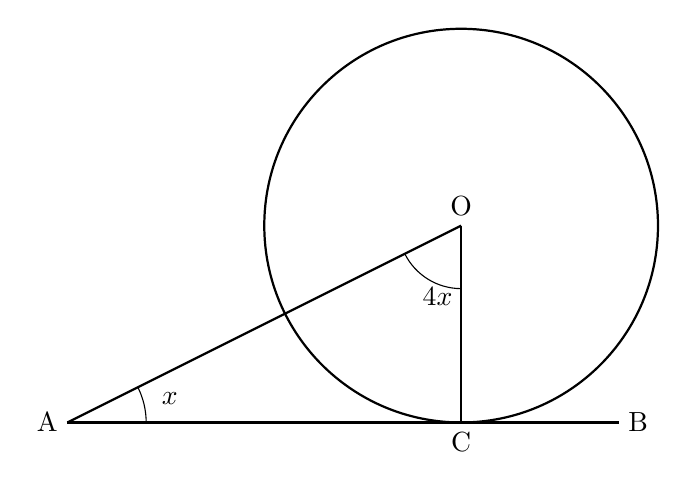
\begin{tikzpicture}[scale=1]

    % --- Coordinates ---
    % A is the external point to the left
    \coordinate (A) at (0,0);
    % C is the point of tangency on the line AB
    \coordinate (C) at (5,0);
    % B is the point on the line to the right
    \coordinate (B) at (7,0);
    % O is the center of the circle, vertically above C
    \coordinate (O) at (5,2.5);

    % --- Drawing the Circle ---
    % Circle centered at O with radius OC
    \draw[thick] (O) circle (2.5);

    % --- Drawing Lines and Segments ---
    % The tangent line through points A, C, and B
    \draw[thick] (A) -- (B);
    % Segment OC (Radius perpendicular to the tangent line)
    \draw[thick] (O) -- (C);
    % Segment AO connecting the external point A to the center O
    \draw[thick] (O) -- (A);

    % --- Arcs for Angles ---
    % Arc for angle x at vertex A
    % atan(2.5/5) is approximately 26.57 degrees
    \draw (1,0) arc (0:26.57:1);
    \node at (1.3,0.3) {$x$};

    % Arc for angle 4x at vertex O
    % Angle is between OC (vertical down, 270 deg) and OA
    \draw (5,1.7) arc (270:206.57:0.8);
    % REPOSITIONED LABEL: Moved 4x down
    \node at (4.7,1.6) {$4x$};

    % --- Point Labels ---
    \node[left] at (A) {A};
    \node[right] at (B) {B};
    \node[below] at (C) {C};
    \node[above] at (O) {O};

\end{tikzpicture}